After clustering the data with a hierarchical clustering algorithm, we developed
a map of the most similar regions according to their cluster. Figure \ref{fig:clustering}
shows these regions. The colors and numbers in Figure \ref{fig:clustering} simply
identify the cluster and do not correspond to heat wave risk nor priority.

\begin{figure}[H]
    \begin{center}
      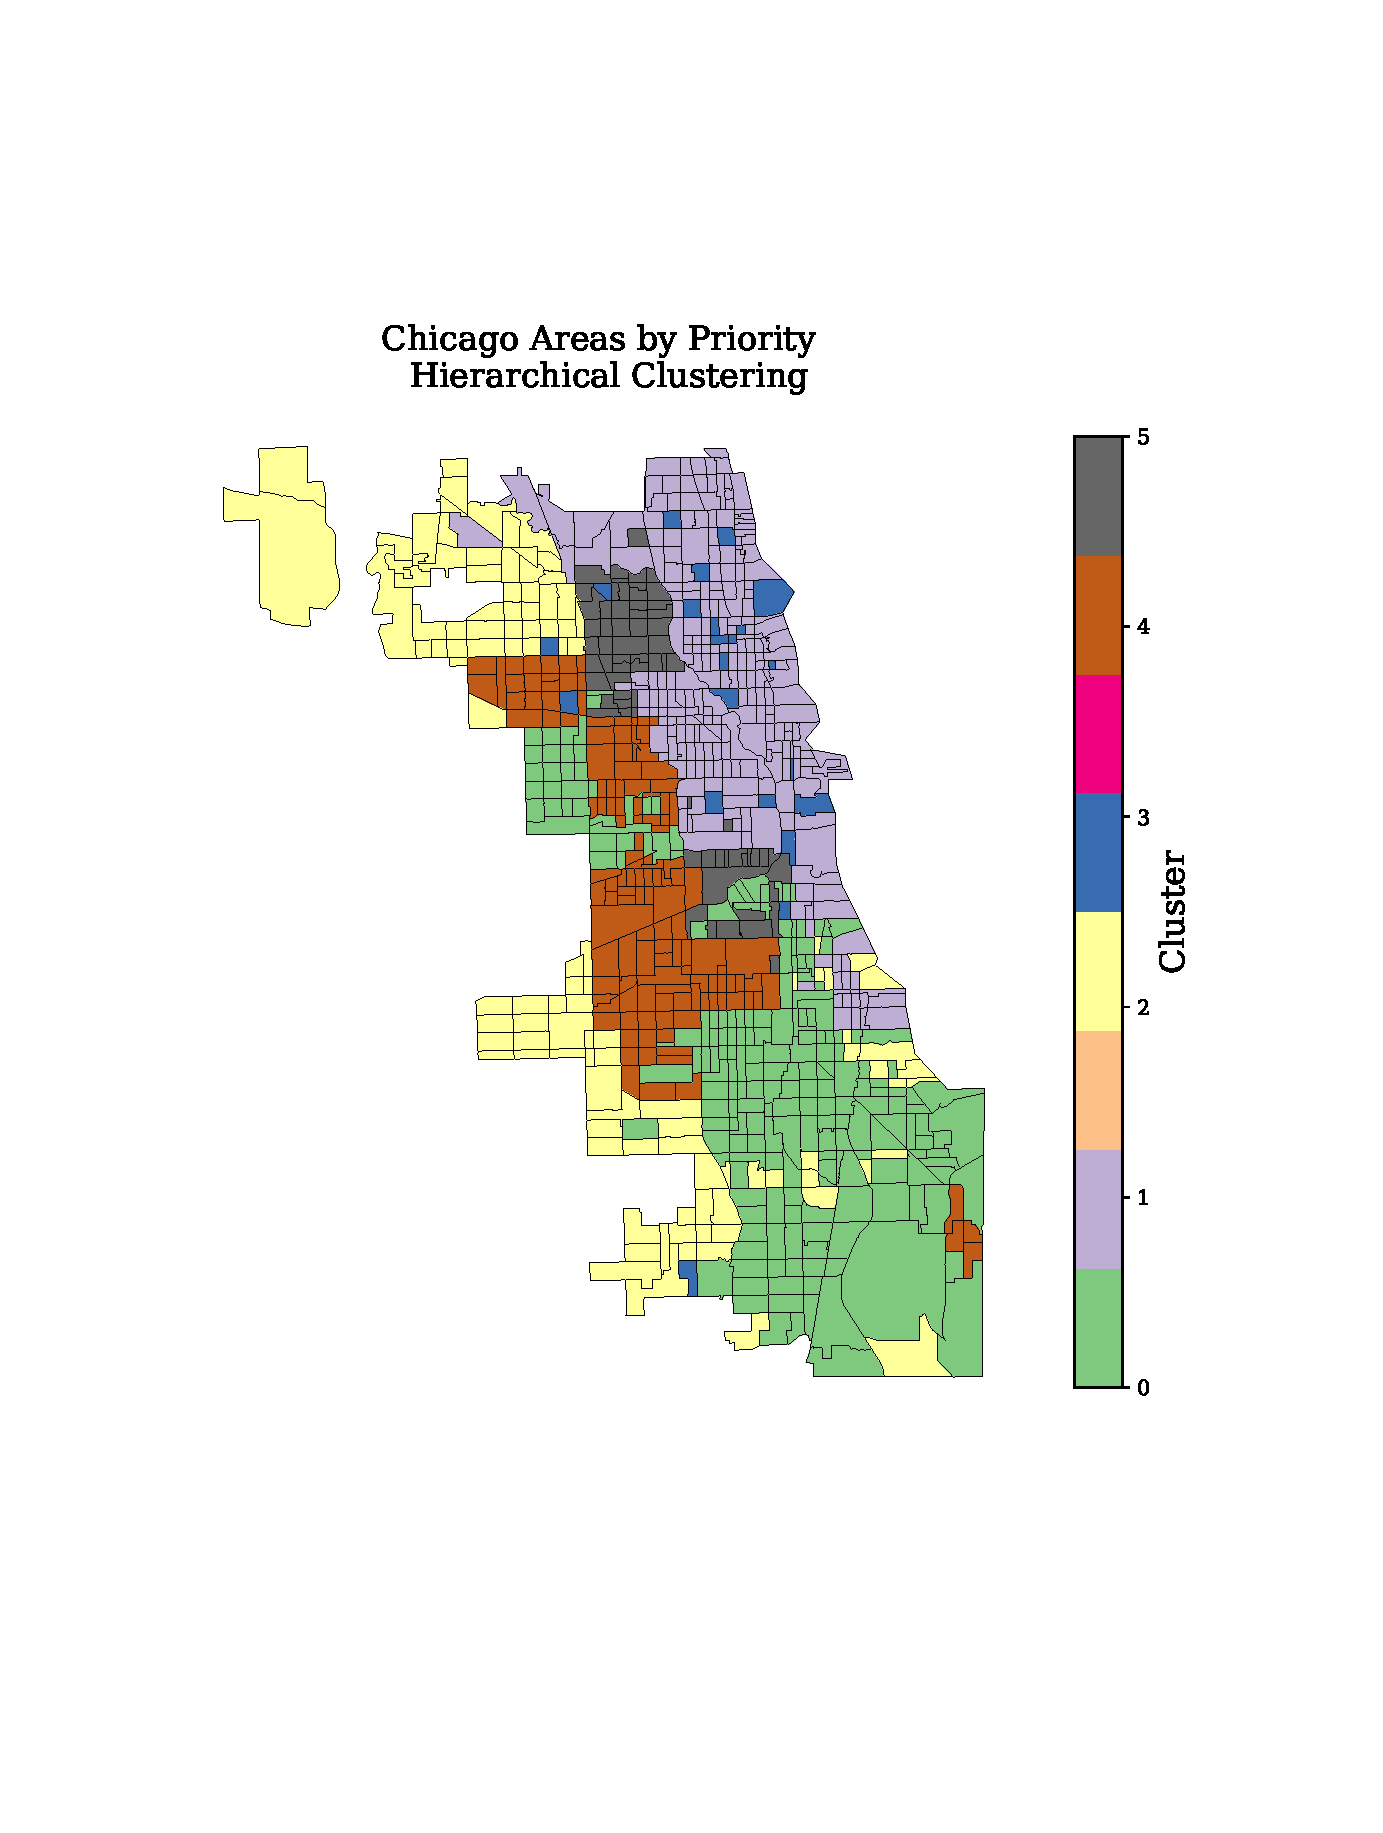
\includegraphics[trim=0 120 0 120, clip, width=\columnwidth]{clustering}
      % \vspace*{-3cm}
      \caption{The map of Chicago clusters. The numbers correspond to the order
      in which the algorithm created the groups and not the heatwave risk.}
      \label{fig:clustering}
    \end{center}
\end{figure}

Figure \ref{fig:cluster_compare} compares the mean vector of each cluster. The
colors and group numbers match the colors and group numbers from Figure
\ref{fig:clustering}.

\begin{figure}[H]
    \begin{center}
      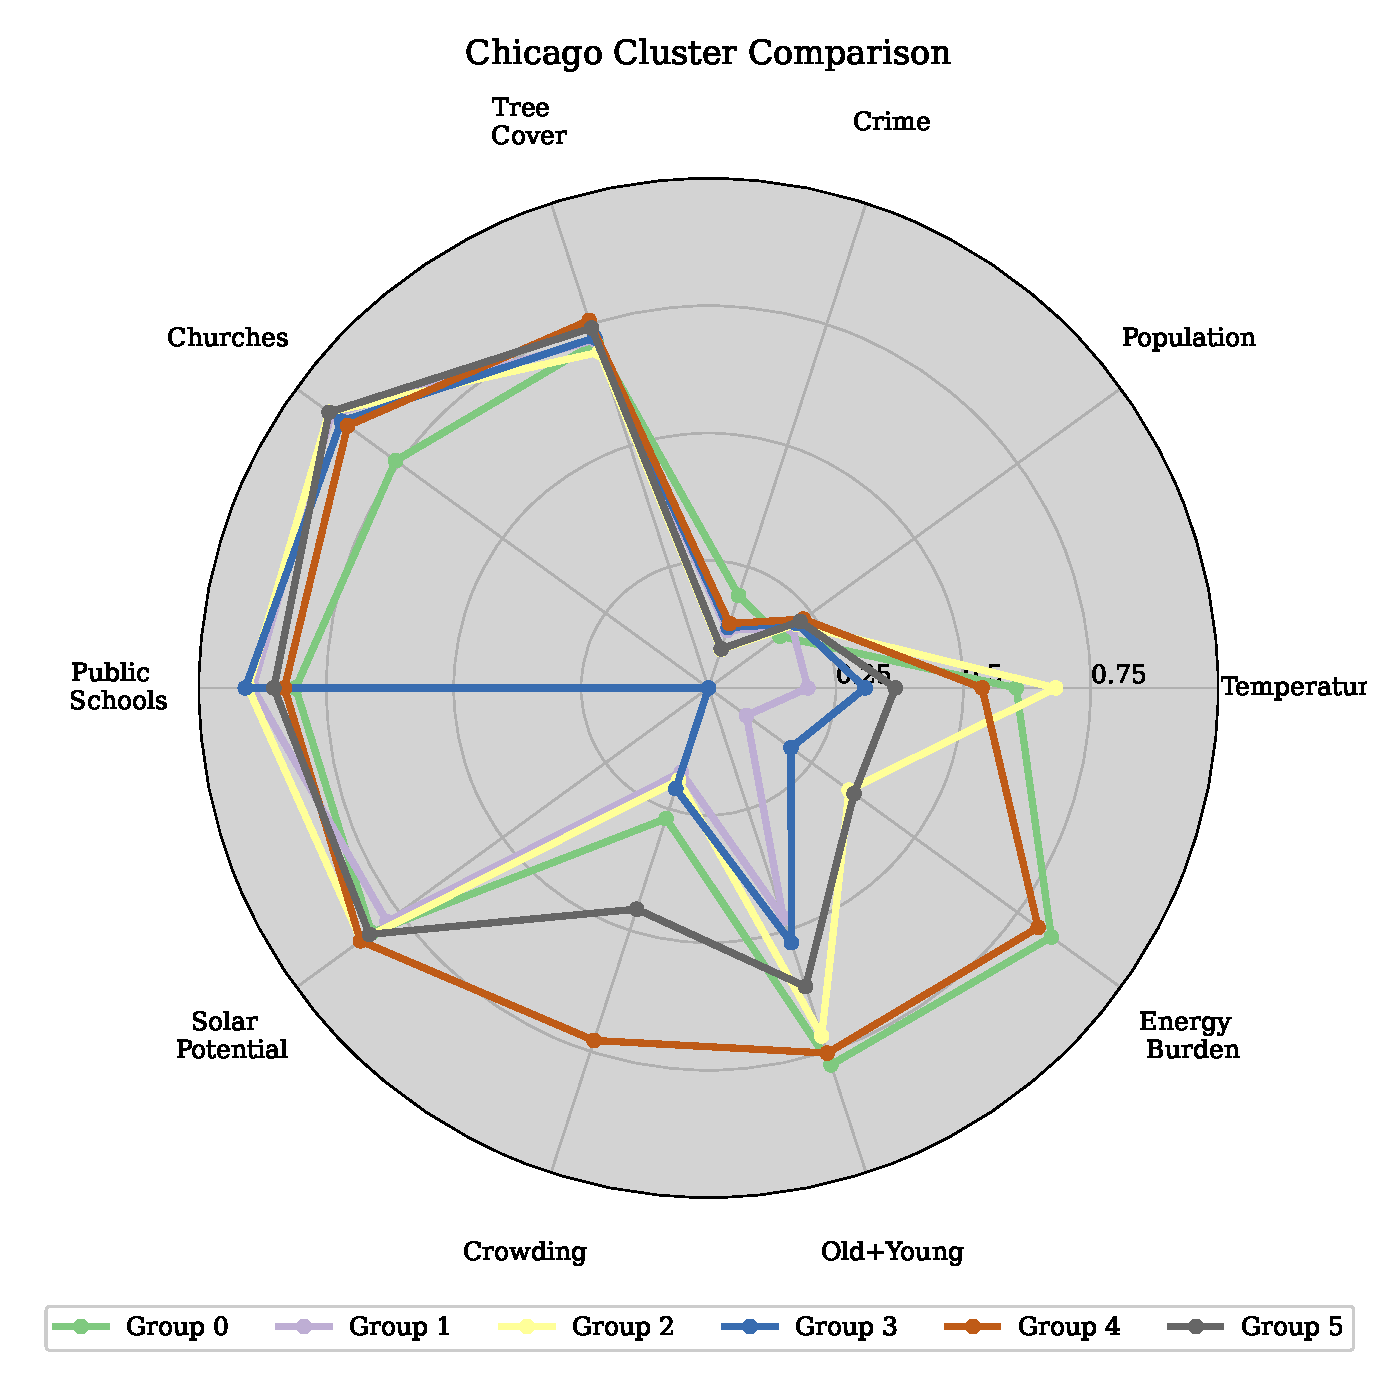
\includegraphics[width=0.95\columnwidth]{cluster_comparison}
      % \vspace*{-3cm}
      \caption{The map of Chicago clusters. The numbers correspond to the order
      in which the algorithm created the groups and not the heatwave risk.}
      \label{fig:cluster_compare}
    \end{center}
\end{figure}

There are several points of interest in Figure \ref{fig:cluster_compare}. First,
the average number of churches, public schools, crime rates, population, and tree
cover were similar across each cluster. The similarity in tree cover was unexpected
due to the strong effect of tree cover on temperature and \ac{uhi} noted in the
literature \cite{mcdonald_tree_2021,marando_urban_2022,schwaab_role_2021}. Further,
there was little difference in average crime rates across clusters. This is likely
due to the fact that a few census tracts had a much higher crime rate than all others.
With the exception of a single group, group 3, solar potential (i.e. the percent
of rooftops that qualify for solar panels \cite{google_project_2022}) was nearly
identical across all clusters.

Second, crowded housing, age, energy burden, and temperature were the most divergent
factors across the clusters. The key difference between the highest and second
highest priority clusters was crowding. It makes sense that the number of people
per household should be used to differentiate priority, \textit{ceteris paribus}.

The ``score'' that ranks the clusters is incidentally the area drawn by each
curve in Figure \ref{fig:cluster_compare}. The rank of each cluster is shown in
Figure \ref{fig:cluster_priority}.

\begin{figure}[H]
    \begin{center}
      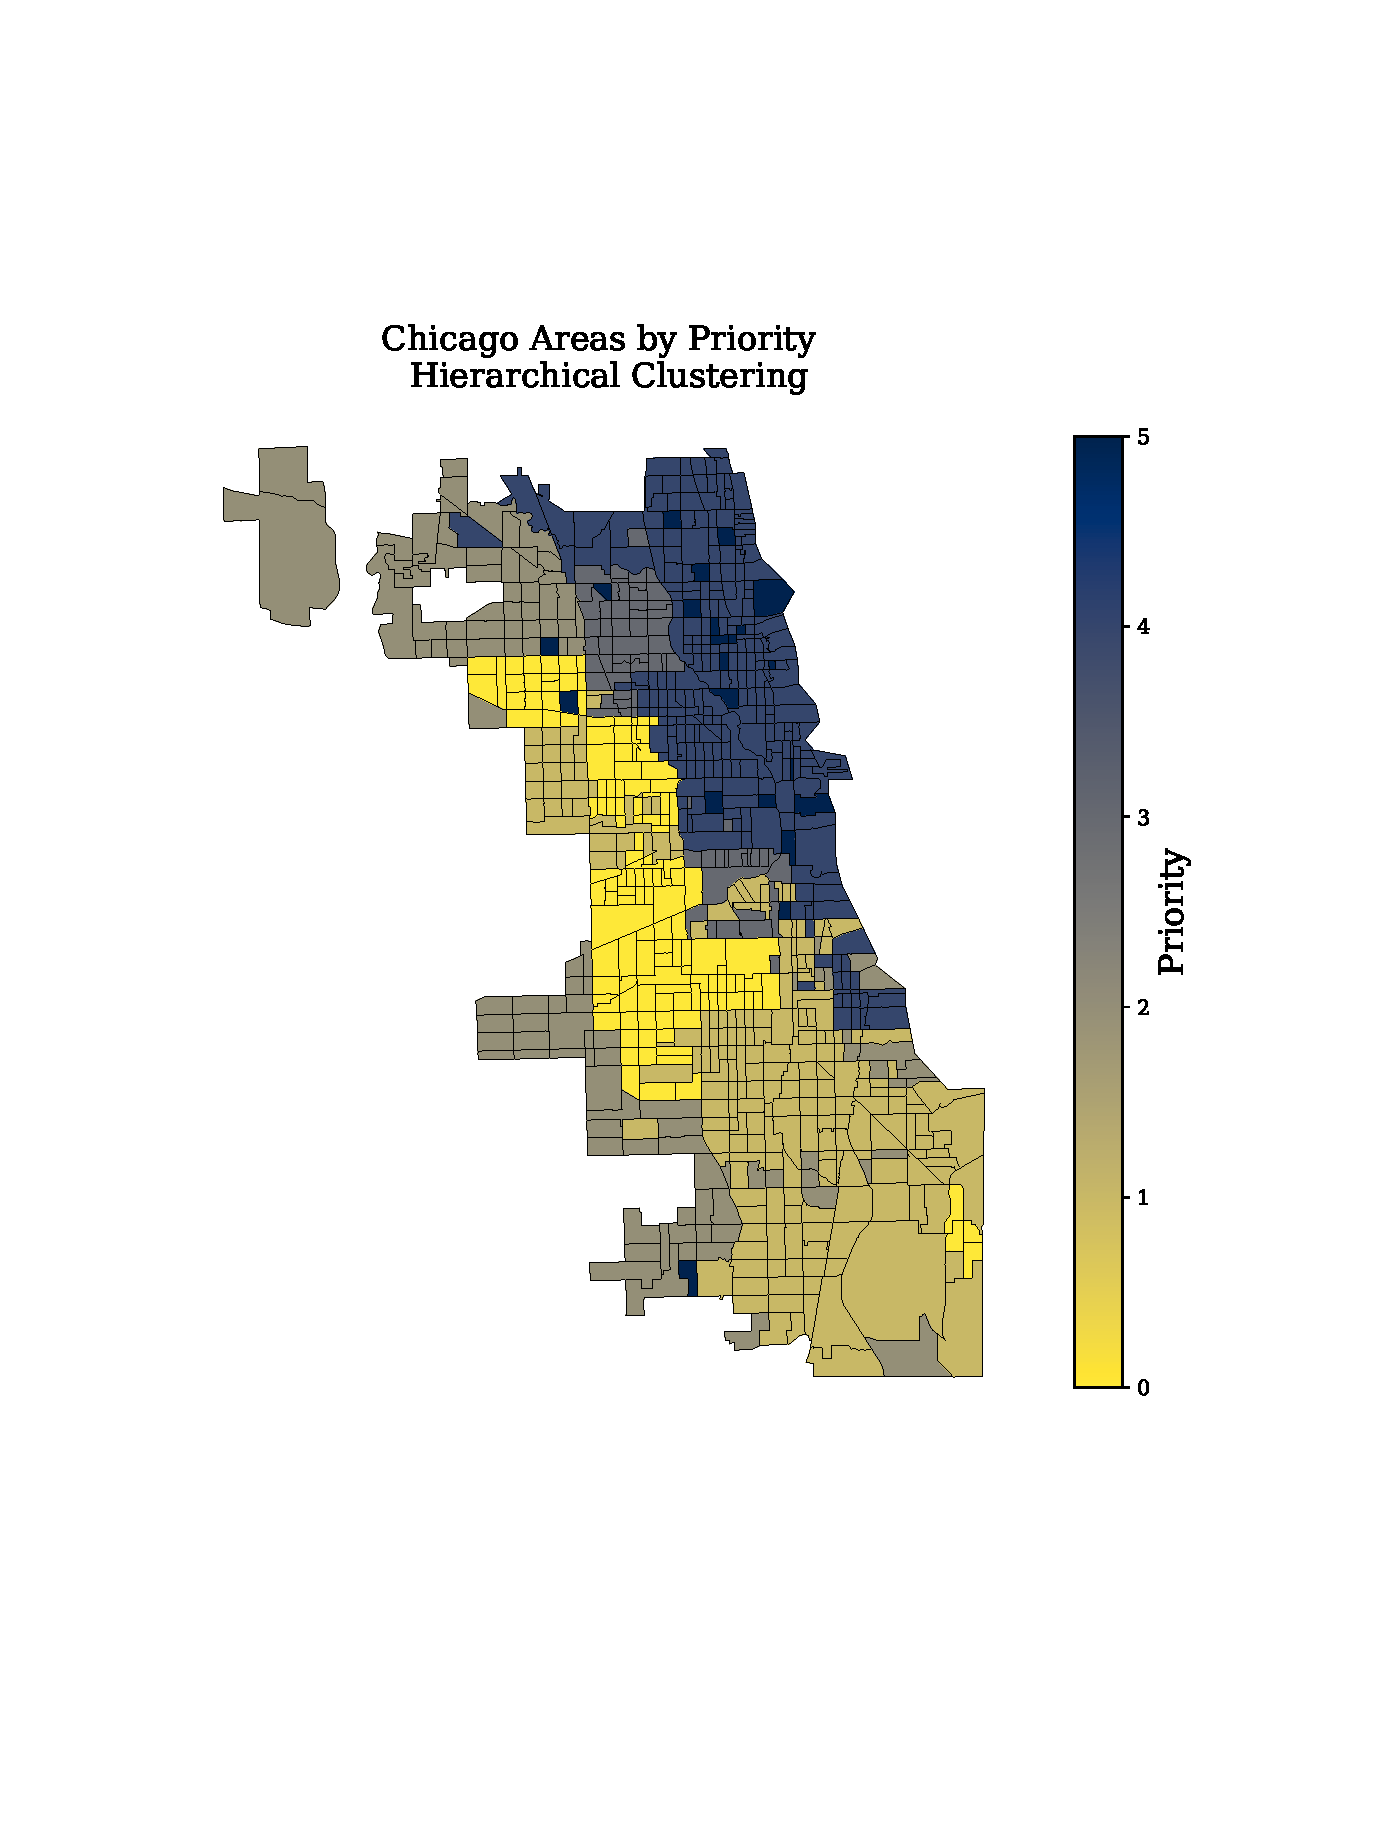
\includegraphics[trim=0 200 0 120, clip, width=\columnwidth]{clustering_priority}
      % \vspace*{-3cm}
      \caption{The map of Chicago clusters according to priority.
      0 = Highest priority. 5 = Lowest priority.}
      \label{fig:cluster_priority}
    \end{center}
\end{figure}

The highest priority region (priority 0) are on the west side of the city, where
it is warmer, crowded, and energy burden is high. The areas closest to Lake Michigan
tend to be the coolest part of the city and the most affluent, thus making them
the lowest priority (priority 5) for rooftop solar panels.
